\section{Participants}
\label{sec:participants}
Participants were recruited from Ontario Tech University's SONA system. 
The study was approved by Ontario Tech's Research Ethics Board (REB), file \#: 17656. 
91 participants completed the study, however 3 were removed due to recording issues, leaving 88 participants.
Signal quality was assessed using the following criteria, similar to \citep{bulgarelli_growth_2025} and \citep{hernandez_nirsplot_2020}: 
Sliding windows of 5 seconds were taken from each channel, and Peak Spectral Power (PSP) and the Scalp Coupling Index (SCI) \citep{pollonini_phoebe_2016} were calculated for each window.
Participants were included in the analysis if they met the following criteria:

\begin{itemize}
    \item If PSP $>$ 0.1 and SCI $>$ 0.5 for more than 70\% of the windows in a single channel, the channel was considered to have good signal quality.
    \item If $>$ 70\% of the channels for a single participant were considered to have good signal quality, the participant was included in the analysis.
\end{itemize}

The minimum SCI threshold was set to 0.5, used in \citep{holmes_opening_2024}, however other studies have used SCI thresholds as low as 0.25 \citep{zhou_autistic_2024}. 
After applying these criteria, 53 participants were included in the analysis. 
All participants met the PSP threshold, but only 53/88 met the SCI threshold, as shown in Figure \ref{fig:signal_quality}.
The 53 participants ranged in age from 17 to 51 (M = 21.60, SD = 6.61), 39/53 were female, and no demographic information was collected. 

\begin{figure}[H]
    \centering
    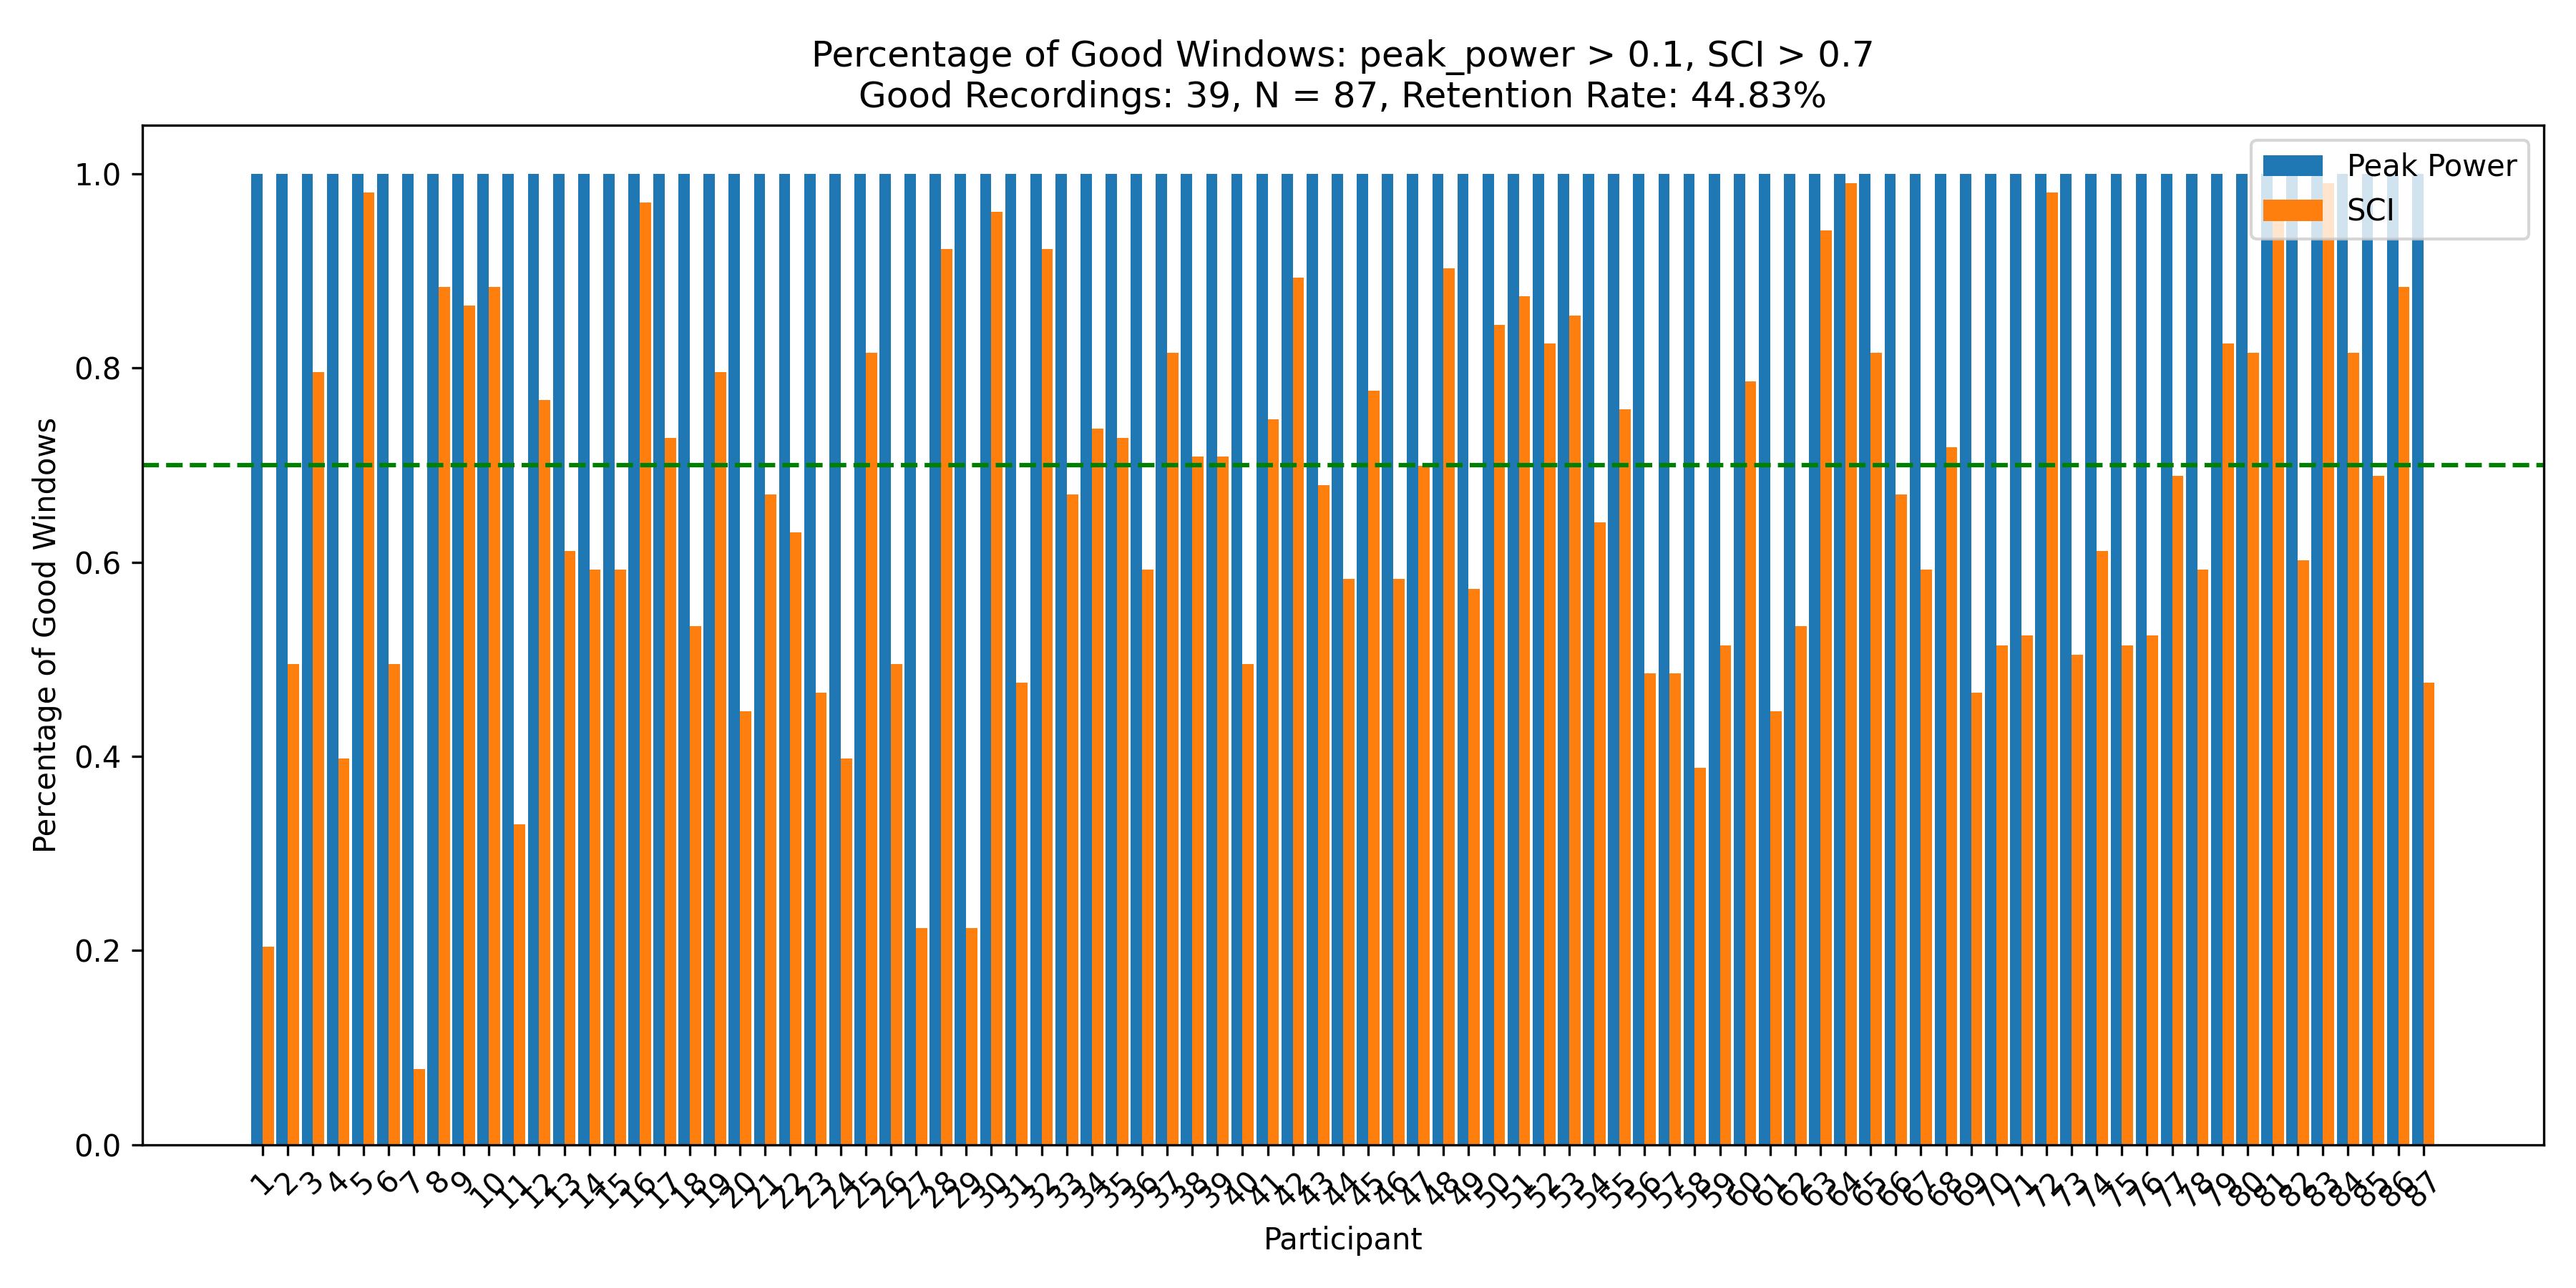
\includegraphics[width=0.9\textwidth]{C:/Users/super/OneDrive - Ontario Tech University/fNIRS_Emotions/plots/signal quality/Percentage of Good Windows.png}
    \caption{Percentage of Channels where SCI $>$ 0.5 for $>$ 70\% of the windows.
    The green dashed line represents the threshold of 70\% of windows that each participant must meet to be included in the analysis.}
    \label{fig:signal_quality}
\end{figure}

\section{Stimuli}
Faces were picked from two datasets: the RADIATE dataset \citep{conley_racially_2018} and the UIBVFED dataset \citep{oliver_uibvfed_2020}. 
The RADIATE dataset is a set of 16 emotional expressions by 109 racially and ethnically diverse real people, aged 18-30 years old.
The UIBVFED dataset is a set of 32 emotional expressions by 20 virtual characters that are also ethnically diverse, aged 20-80 years old.
To create the UIBVFED faces, the authors used blendshapes, which is an effective way to represent facial action units \citep{ekman1978facial}. 
The faces used in the stimuli presentation were picked carefully, then validated by both co-supervisors with this strict criteria in mind:
\begin{itemize}
    \item 20 young adult models were selected, 5 males, 5 females from both datasets (RADIATE and UIBVFED). 
    \item The corresponding models from each dataset were matched as closely as possible, in terms of each model's face shape, sex, skin tone, and hair color. 
    \item 7 emotional expressions (anger, disgust, fear, happiness, sadness, surprise, neutral) were selected for each model, that closely align with Ekman's 6 basic emotions + neutral \citep{ekman_are_1992}.
\end{itemize}

The final dataset consisted of 10 models from the RADIATE dataset and 10 models from the UIBVFED dataset, with 7 emotional expressions for each model, and each model had a corresponding model in the other dataset that matched them as closely as possible.
The RADIATE dataset was used for the real faces, and the UIBVFED dataset was used for the virtual faces.
The UIBVFED images were cropped to the same size as the RADIATE images, for consistency in the stimuli presentation.

\section{Design and Procedure}
\subsection{Design}
We used a repeated-measures design consisting of five within-subjects factors:

\begin{itemize}
    \item \textbf{Face Type}: 2 levels (Real, Virtual)
    \item \textbf{Emotion}: 7 levels (Anger, Disgust, Fear, Joy, Sadness, Surprise, Neutral)
    \item \textbf{Model}: 10 unique identities per face type
    \item \textbf{Sex}: 2 types of models per face type (Male, Female)
    \item \textbf{Repetition}: 28 repetitions of each Face Type, 8 repetitions of each Emotion
\end{itemize}

This yielded 56 blocks, each comprising eight faces (4 male, 4 female) of the same face type and emotional expression, counterbalanced across Face Type and Emotion.

\subsection{Procedure}
\label{sec:Procedure}
Upon entering the lab, the participant was greeted by the experimenter and asked to read and sign a consent form. 
Their head size was then measured using a tape measure, and the fNIRS cap was fitted to their head as the fNIRS cap was explained to them.
The participant waited patiently while the experimenter(s) checked the signal quality in Aurora fNIRS, the acquisition software for the NIRSport2 system.
The experimenter(s) then attempted to move the participants' hair out of the way of the optodes, to improve signal quality.
The experimenter(s) then explained the task to the participant, and notified them of the camera/microphone in the back of the room. 
No emphasis was given on what to focus on during the task, all the participant was told is that they will be seeing many different types of faces, and that they need to complete the memory task, which is as follows:

\subsubsection{Memory Task:}
\label{sec:memory_task}
The participant will see blocks of 8 faces, and after each block, there will be a 9th face, and they will need to indicate whether the 9th face was in the previous block of 8 faces.
The participant was instructed to press 'y' on the keyboard if the face was in the previous block, or 'n' if the face was not in the previous block.
This task is visualized in Figure \ref{fig:paradigm}. 

The experimenter(s) then turned the lights off in the room to avoid any interference with the fNIRS cap. 
Then the experimenter(s) started the experiment, and left the room to minimize noise and distractions.
Experimenter(s) then monitored the experiment from outside the room. 
After the experiment was completed (about 35 minutes later), the experimenter(s) entered the room, removed the fNIRS cap, and the participant was given a debriefing letter to read and take home. 
The main purpose of the memory task was to keep the participant engaged and focused on the faces, the memory task was not the main focus of the study, and this was divulged to the participant if they inquired about it after the experiment was completed.

\begin{figure}[H]
    \centering
    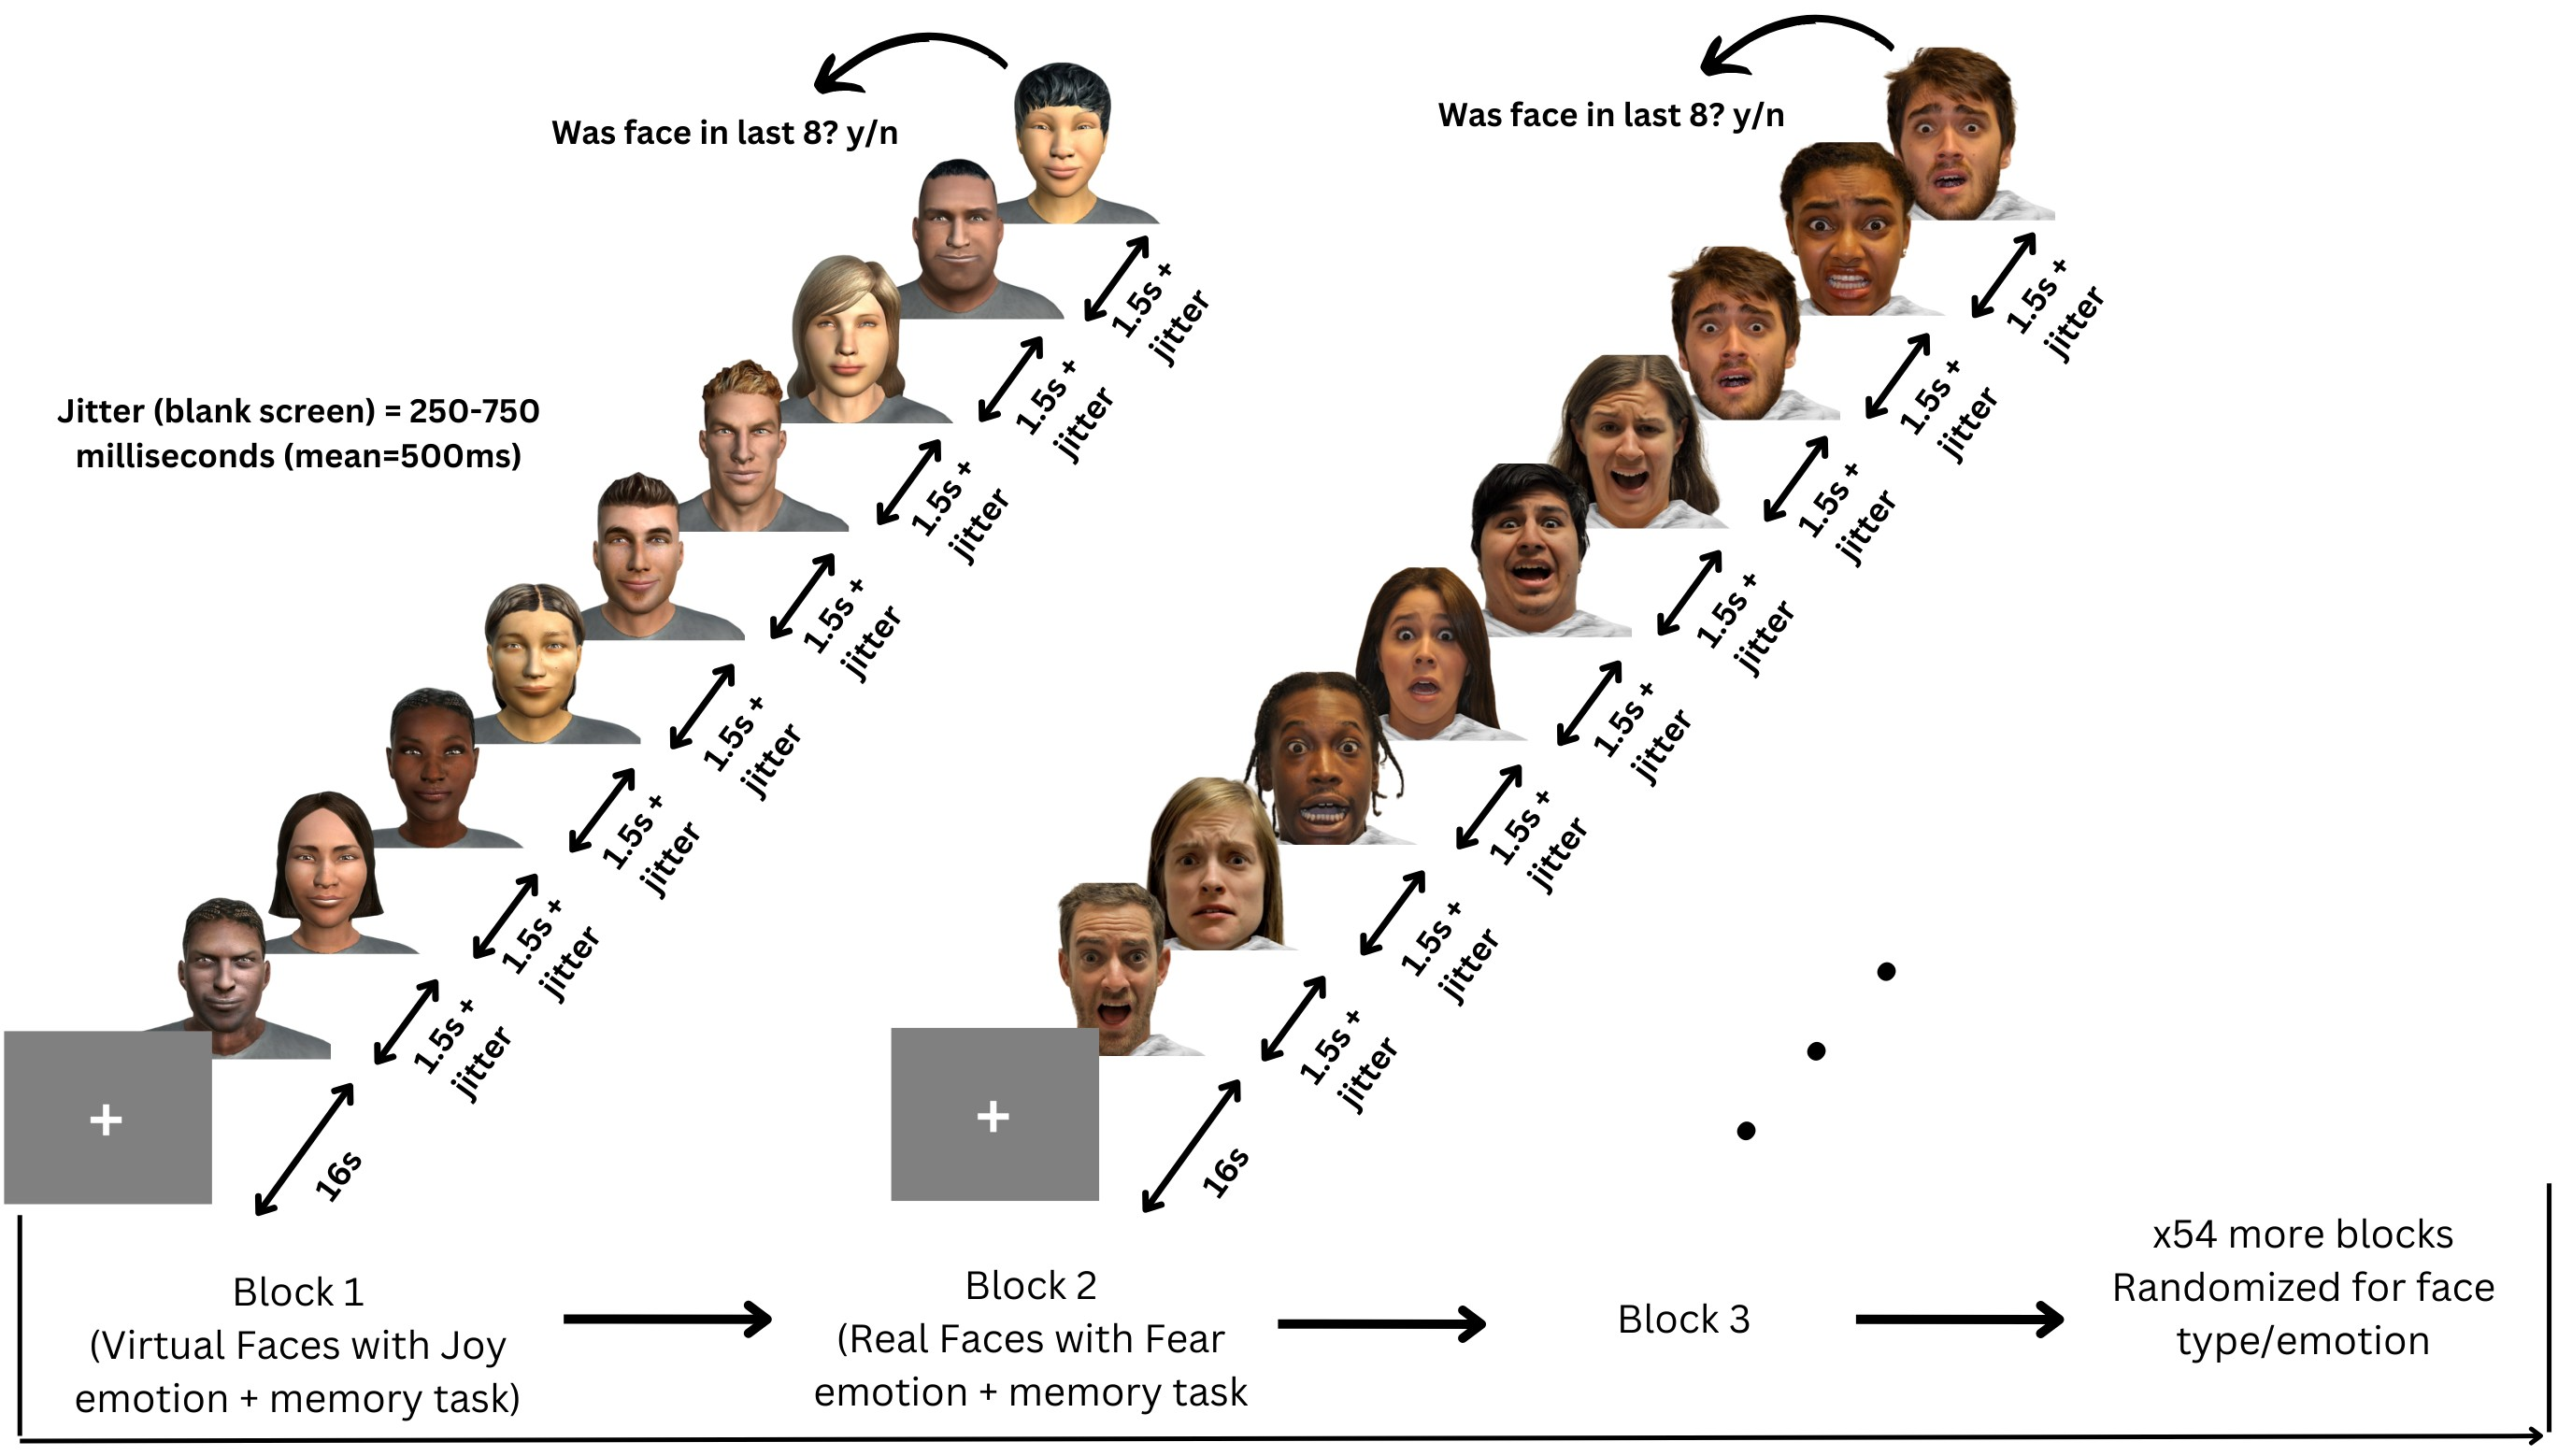
\includegraphics[width=0.9\textwidth]{C:/Users/super/OneDrive - Ontario Tech University/fNIRS_Emotions/plots/figures/Paradigm.jpg}
    \caption{Participants viewed 56 blocks of 8 faces, each block being either all real or all virtual faces.
    Every face in a block displayed the same emotional expression, one of: anger, disgust, fear, happiness, sadness, surprise, neutral. }
    \label{fig:paradigm}
\end{figure}

The stimuli presentation was prepared using PsychoPy3 Experiment Builder (v2024.1.5) \citep{peirce_psychopy2_2019}. 
The stimuli were presented on a Dell U2415 24 inch 1920x1200 60Hz monitor, placed at eye level, and the participants were seated in a comfortable chair facing the monitor.
The beginning of the stimuli presentation had instructions on the screen, which explained the task to the participant, and the participant entered the space bar when they were ready to start the experiment.

The format of the stimuli presentation was as follows: There are 56 blocks in total, each block consists of 8 faces followed by a 9th face.
The faces within each block are either real (from the RADIATE dataset) or virtual (from the UIBVFED dataset), and the faces are presented in a random order.
All faces within a block had one of seven emotional expressions (joy, fear, anger, disgust, sadness, neutral, surprise), and all faces within a block express the same emotion. 
Between every block and starting the experiment, there is a fixation cross presented for 16 seconds. 
The 8 faces (4 male, 4 female, randomly selected) are presented one at a time, for 1.5 seconds each, with a 250-750 ms (mean 500 ms) interstimulus interval (ISI) between each face. 
The 9th face is presented after the 8th face, and the participant must indicate whether the 9th face was in the previous block of 8 faces by pressing 'y' for yes or 'n' for no. 
This task is described in detail in section \ref{sec:memory_task}.
The 9th face has a 50\% chance of either being in the previous block or not, and if the participant does not respond within 7 seconds, the presentation will continue to the next block.
Every 7 blocks, the participants are given a break, and prompted to enter the space bar when they are ready to continue the experiment.
The stimuli presentation lasted approximately 35 minutes in total. 
This paradigm is shown in Figure \ref{fig:paradigm}.

\section{Data Acquisition}
fNIRS data was collected using two NIRSport2 systems (NIRx Medical Technologies, Berlin, Germany). 
Each NIRSport2 system was equipped with 16 source and 16 detector optodes, and daisy-chained together for a high density 32x32 optode configuration. 
Each neighboring pair of source and detector optode is referred to as a channel, resulting in a total of 103 HbO + 103 HbR channels (plus 16 short distance channels).
The average distance between source and detector optodes was 30 mm, and 7mm for short distance channels, which were placed on a flexible fNIRS head cap (NIRScap) 58 cm in circumference. 
The optodes were arranged in a high density 32x32 montage with one bundle of short distance channels, as shown in Figure \ref{fig:montage_combined}.
This montage was designed to cover a maximally large area of the brain, given increasing evidence that emotion processing is not localized to specific discrete areas of the brain, rather distributed across the brain \citep{lindquist_brain_2012}. 
The fNIRS cap and optodes were positioned following the 10-20 international coordinate system.
Light was emitted at 760 nm and 850 nm wavelengths, and the sampling rate was approximately 6.105 Hz.

\begin{figure}[H]
    \centering
    \begin{subfigure}[b]{0.9\textwidth}
        \centering
        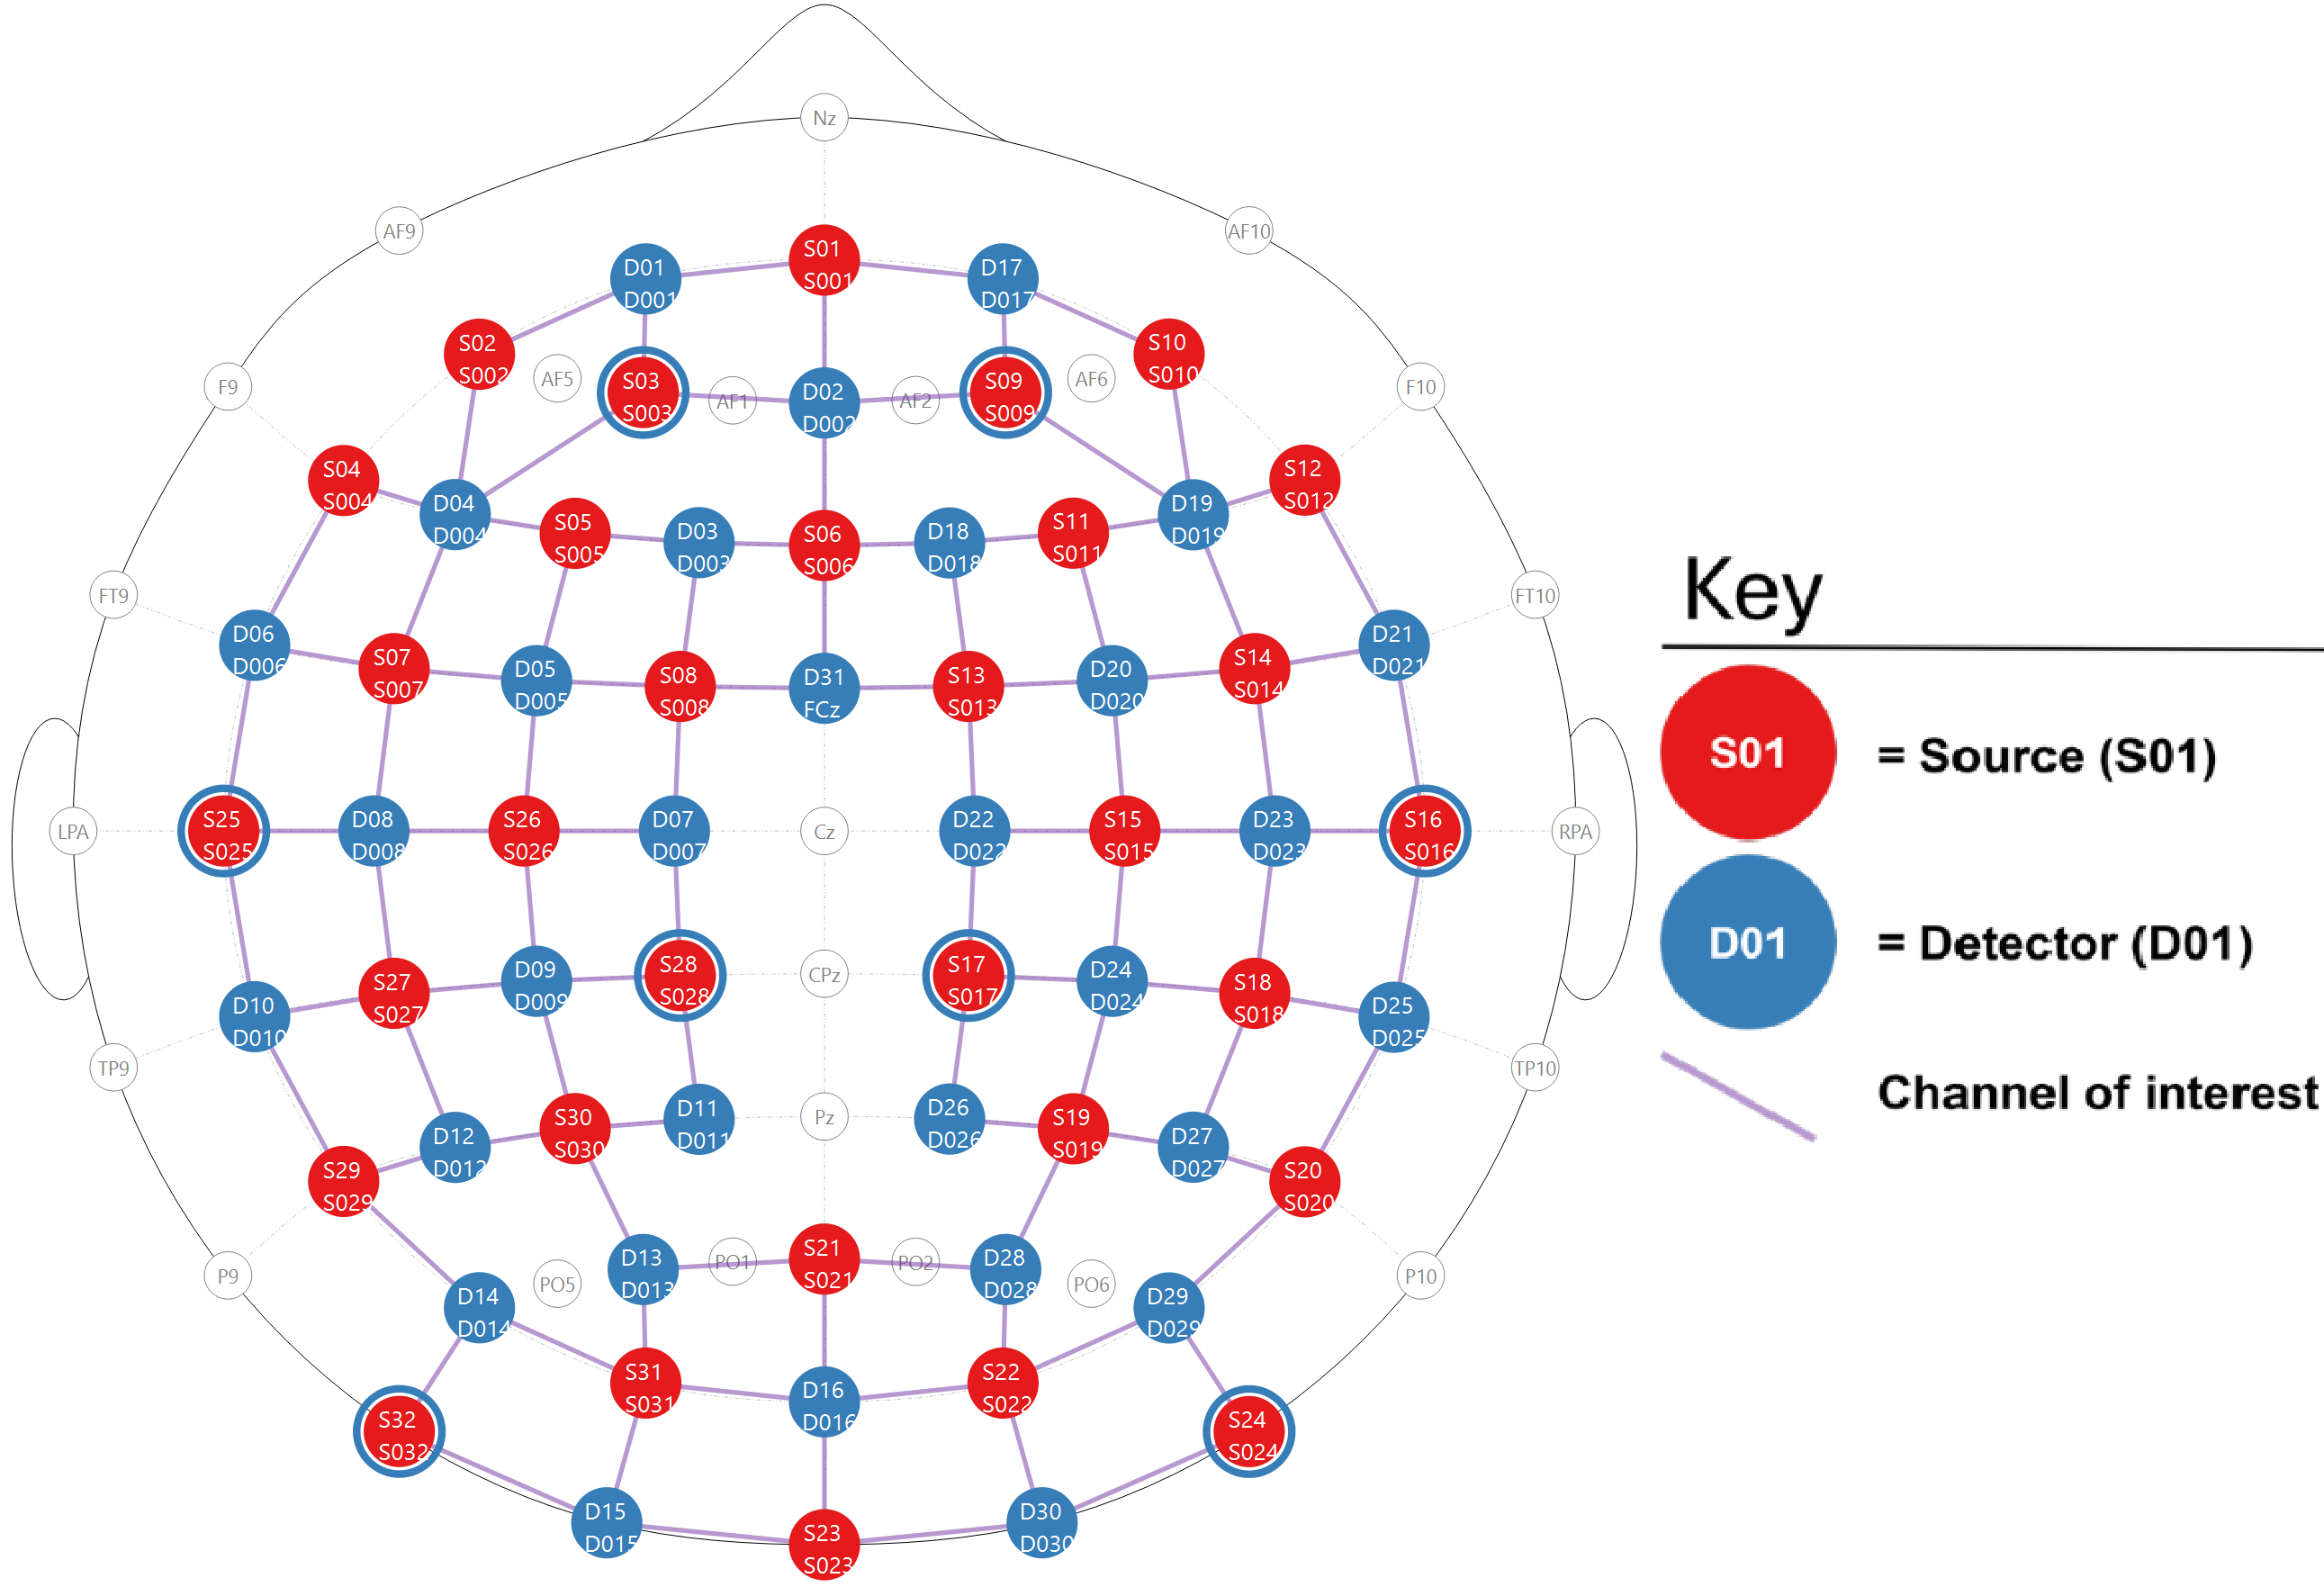
\includegraphics[width=\textwidth]{C:/Users/super/OneDrive - Ontario Tech University/fNIRS_Emotions/plots/figures/Montage.png}
        \caption{2D depiction of the montage. }
        \label{fig:montage_2d}
    \end{subfigure}
    \hfill
    \begin{subfigure}[b]{0.45\textwidth}
        \centering
        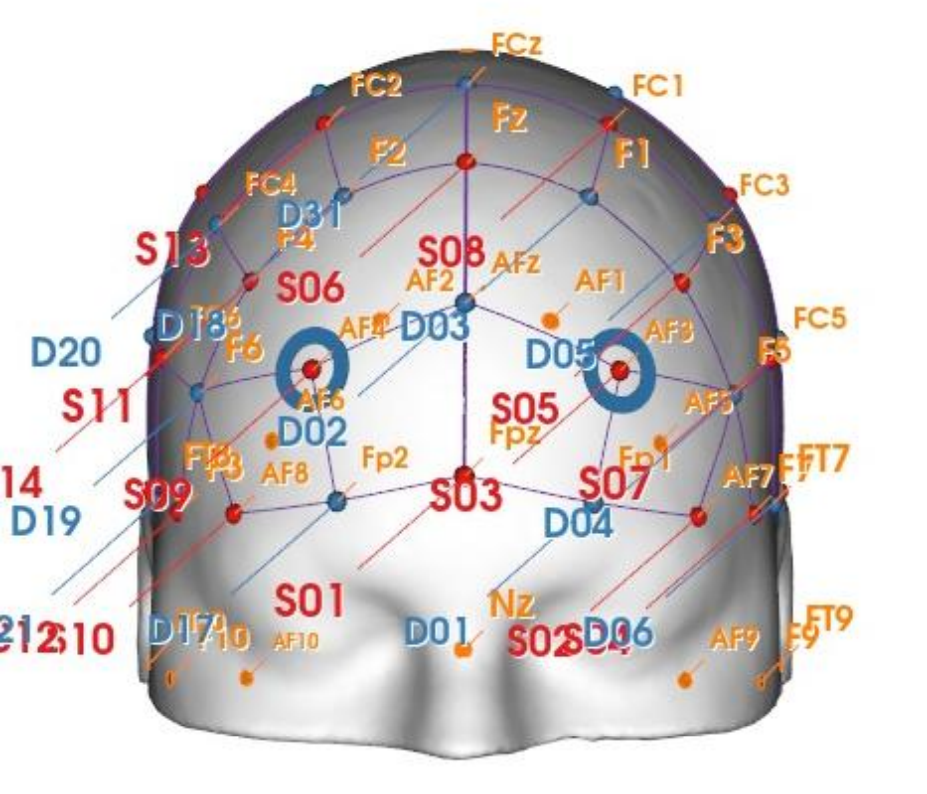
\includegraphics[width=\textwidth]{C:/Users/super/OneDrive - Ontario Tech University/fNIRS_Emotions/plots/figures/Montage Front View.png}
        \caption{3D front view of the montage.}
        \label{fig:montage_front}
    \end{subfigure}
    \hfill
    \begin{subfigure}[b]{0.45\textwidth}
        \centering
        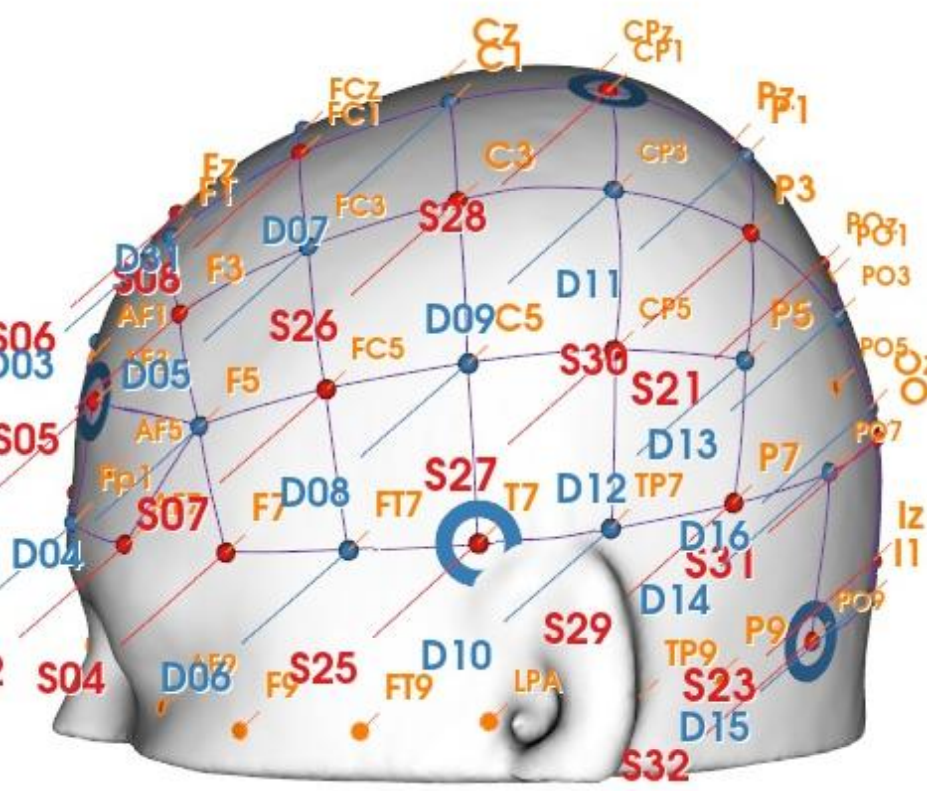
\includegraphics[width=\textwidth]{C:/Users/super/OneDrive - Ontario Tech University/fNIRS_Emotions/plots/figures/Montage Side View.png}
        \caption{3D side view of the montage.}
        \label{fig:montage_side}
    \end{subfigure}
    \caption{Depictions of the high density 32x32 optode montage. Red circles represent sources, blue circles represent detectors, purple lines represent channels, and blue rings around sources represent the locations of the 8 short distance detectors.}
    \label{fig:montage_combined}
\end{figure}

\section{Analysis}
All fNIRS data was preprocessed and analyzed with Python 3.11.9 using MNE (version 1.9.0) \citep{gramfort_meg_2013} and MNE-NIRS (version 0.7.1) \citep{luke_analysis_2021}, which used the Nilearn package (version 0.9.2). 
First, the General Linear Model (GLM) analysis was performed, followed by a Functional connectivity analysis. 
Both analyses were performed on the same set of data collected from \ref{fig:paradigm}, and the memory task analysis was performed on the y/n responses from the memory task.

\subsection{Preprocessing Steps}
\begin{figure}[H]
    \centering
    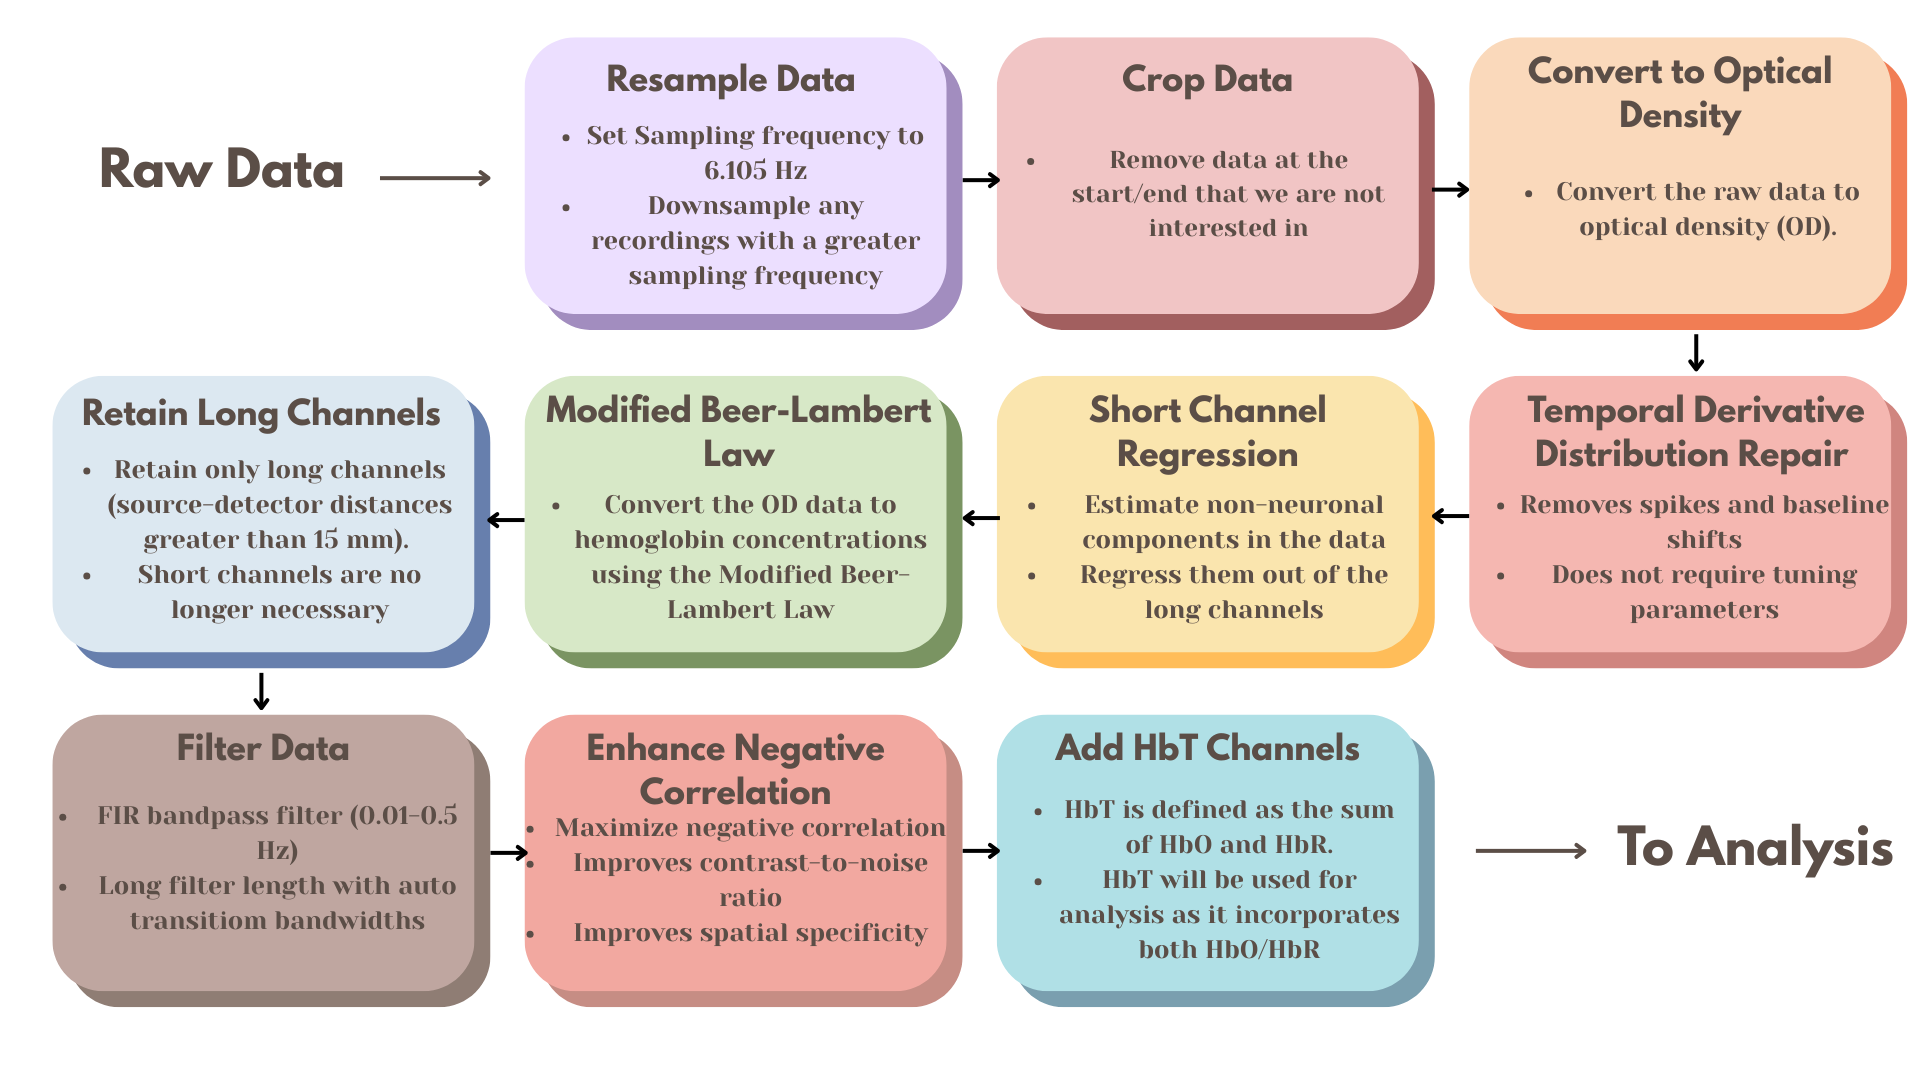
\includegraphics[width=0.9\textwidth]{C:/Users/super/OneDrive - Ontario Tech University/fNIRS_Emotions/plots/figures/Preprocessing Steps.png}
    \caption{Preprocessing steps for fNIRS data, from the raw data to the fully processed data. }
    \label{fig:preprocessing_steps}
\end{figure}

\begin{enumerate}
    \item \textbf{Downsample Data:} Downsample the data if the sampling frequency is greater than 6.105 Hz, the initial two datasets were sampled higher than 6.105 Hz, and the sampling frequency should be consistent across all datasets.
    \item \textbf{Crop Data:} Crop the data to the first and last annotation. This gets rid of the extra data at the beginning and end of the recording that are not of interest.
    \item \textbf{Convert to Optical Density (OD):} Convert the raw data to optical density.
    \item \textbf{Temporal Derivative Distribution Repair (TDDR):} Apply temporal derivative distribution repair to the OD data \citep{fishburn_temporal_2019}. TDDR is effective at removing spikes and baseline shifts from the data. 
    \item \textbf{Short Channel Regression:} Apply short channel regression to the OD data \citep{scholkmann_measuring_2014}. Short channels are used to estimate the superficial hemodynamics (non-evoked/extracerebral/systemic components) in the data, and then regress it out of the long channels \citep{tachtsidis_false_2016}. 
    \item \textbf{Modified Beer-Lambert Law (MBLL):} Convert the OD data to hemoglobin concentrations using the modified Beer-Lambert law. The MBLL relates the change in light attenuation to the change in hemoglobin concentration of chromophores in the tissue \citep{kocsis_modified_2006}.
    \item \textbf{Retain Long Channels:} Retain only long channels (source-detector distance $>$ 15 mm). Since the short channels have already been regressed out, it is no longer necessary to keep them in the data.
    \item \textbf{Filter Data:} This FIR bandpass filter extracts signal components in the 0.01-0.5 Hz range, it uses a long filter length (2015 samples) with automatically determined transition bandwidths by MNE-Python \citep{pinti_current_2019}. 
    \item \textbf{Enhance Negative Correlation:} Maximizes negative correlation between HbO and HbR \citep{cui_functional_2010}. This method removes spikes, improves contrast-to-noise ratio, and improves spatial specificity of the data.
    \item \textbf{Add HbT Channels:} Add HbT (hemoglobin total) channels to the data. HbT is defined as the sum of HbO and HbR. Often, fNIRS studies will only use either one of HbO or HbR channels (more frequently HbO), leaving out one channel with no justification \citep{kinder_systematic_2022}. Therefore, HbT channels are chosen, as HbT makes use of both HbO and HbR channels, and using both hemoglobin species improves the inferences as to where activation occurs \cite{hocke_automated_2018}.
\end{enumerate}

\subsection{Epochs}
Variable length epochs were created for each block of 8 faces, each block was 14-18 seconds long (mean = 16s), depending on the ISI's as described in \ref{sec:Procedure}.
Epochs were sorted by Face Type (Real, Virtual), and Emotion (Anger, Disgust, Fear, Happiness, Sadness, Surprise, Neutral). 
Baseline correction was applied to remove any constant or slowly varying offsets in the data. 
The data was annotated with the onsets and offsets of each block, along with the duration and condition of each block for use in section \ref{sec:GLM} and \ref{sec:connectivity_analysis}.

\subsection{General Linear Model (GLM) Analysis}
\label{sec:GLM}
The General Linear Model (GLM) posits that the observed haemodynamic signal at each channel or Region of Interest (ROI) is a linear combination of task-related regressors convolved with a Hemodynamic Response Function (HRF), plus nuisance regressors (e.g., drift) and residual noise. Mathematically, 

\begin{equation}
Y = X\beta + \epsilon,
\end{equation}

where \( Y \) is the observed time series, \( X \) is the design matrix, \( \beta \) represents the parameters to estimate, and \( \epsilon \) denotes the residuals assumed to be (i.i.d.) Gaussian noise.
Estimation is performed via ordinary least squares (OLS), yielding parameter estimates that quantify condition-specific activation amplitudes.

\subsubsection{Design Matrix}
For each of the epochs, events are defined by their trial type (e.g., emotion or face type), and onsets/offsets relative to the procedure start, and duration.
The design matrix is constructed using Nilearn's \texttt{make\_first\_level\_design\_matrix} by convolving a boxcar function (based on the event timing) with a canonical HRF, which is a model of the expected haemodynamic response to neural activity.
The canonical HRF Statistical Parametric Mapping (SPM) \citep{friston_statistical_2007} is chosen to model neurovascular coupling, this model captures the stereotypical rise and fall of the BOLD/fNIRS response. 
The cosine drift model was utilized, which incorporates discrete cosine transform (DCT) basis functions into the design matrix to model and remove low-frequency drifts.
The selection of the high pass cutoff frequency is guided by the structure of the experimental design. 
The cutoff period is set to twice the duration of the longest inter-trial interval, and each fixation period between epochs (or blocks) is 16 seconds. 
Therefore, a cutoff period of 32 seconds (i.e., \texttt{high\_pass=0.03125} Hz) would be appropriate. 
This ensures that the drift model does not remove task-related signal components that occur at frequencies higher than the cutoff \citep{luke_analysis_2021}.
The design matrix \( X \) and preprocessed time series are fed into MNE's \texttt{run\_glm} function, which computes OLS estimates of \( \beta \) for each channel.

\begin{figure}[H]
    \centering
    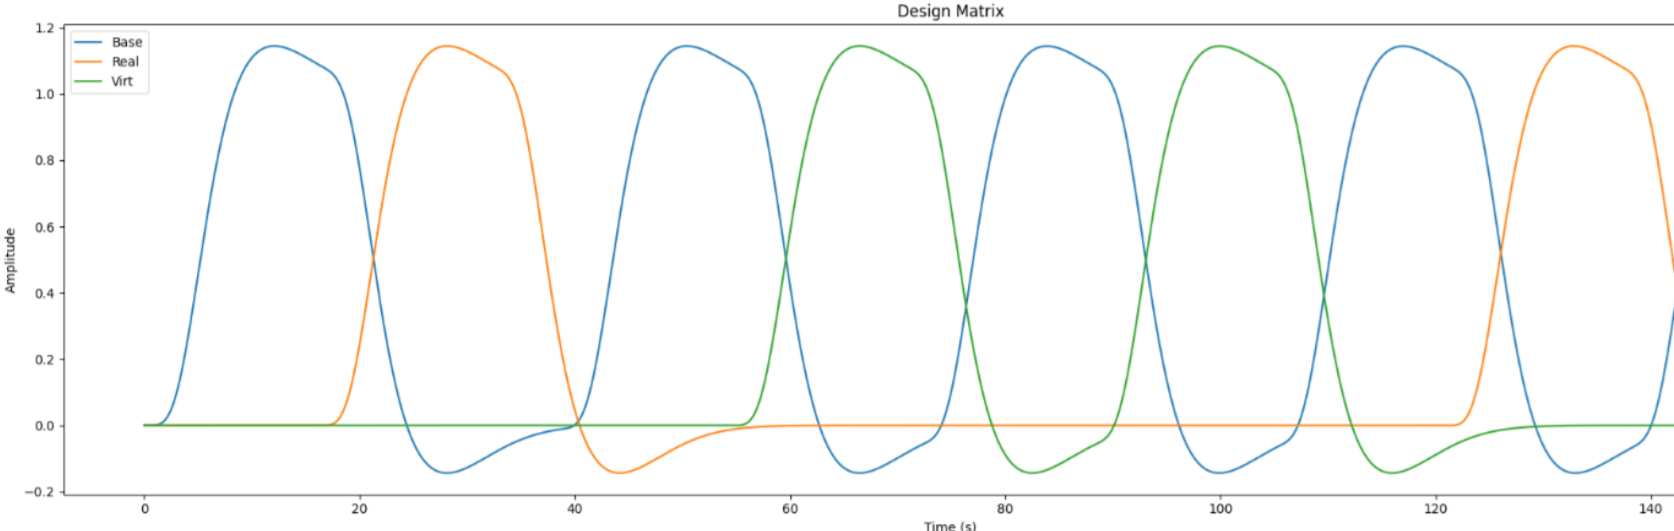
\includegraphics[width=1\textwidth]{C:/Users/super/OneDrive - Ontario Tech University/fNIRS_Emotions/plots/figures/Sample Design Matrix.png}
    \caption{Sample design matrix for a single participant for the effect Face type, showing the first 7 blocks (250 seconds) of a single experiment.
    The design matrix is organized by condition (Blue for real, orange for virtual), this is the result of convolving the boxcar function with the canonical HRF SPM. }
    \label{fig:design_matrix}
\end{figure}

\subsubsection{Contrast Computation}
\label{sec:contrast_computation}
All pairwise contrasts were generated between conditions by constructing an identity contrast matrix over design columns. 
For each pair of conditions \( (A, B) \), the contrast vector is defined as: $c = e_A - e_B$, where \( e_A \) and \( e_B \) are the respective design matrix columns for conditions \( A \) and \( B \). 
Contrasts are computed using MNE's \texttt{compute\_contrast} function, which produces effect estimates and test statistics aggregated across channels.
Since numerous statistical tests are performed across channels and contrasts, $p$-values were corrected for false discovery rate (FDR) using the Benjamini-Hochberg procedure \citep{singh_exploring_2006} with a family-wise error rate of $\alpha$=0.05.

\subsection{Functional Connectivity Analysis}
\label{sec:connectivity_analysis}
In order to characterize the temporal coordination between fNIRS channels during emotional face processing, functional connectivity matrices were computed using a continuous wavelet transform (CWT)-based spectral connectivity approach.
CWT decomposes signals into simultaneous time-frequency representations, providing an optimal framework for fNIRS connectivity analysis by accommodating the non-stationary, physiological nature of hemodynamic signals. 
The morlet wavelet, a gaussian function modulated by a sine wave, was picked as they are suited to capture both slow neural rhythms and faster systemic fluctuations in fNIRS data \citep{reddy_evaluation_2021}. 
Wavelet-based approaches have been widely adopted in the fNIRS literature for connectivity and even artifact correction \citep{bergmann_evaluation_2023}. 
Approximately 90 fNIRS studies employ wavelet coherence to map dynamic inter-regional coupling during tasks or resting-state \citep{hakim_quantification_2023}.
Coherence combines both phase and amplitude information into a single, normalized index, 0 (no coupling) to 1 (perfect coupling), and is a richer description of coupling than phase-only or amplitude-only metrics \citep{bastos_tutorial_2016}.
For each participant, MNE's \texttt{spectral\_connectivity\_time} function was applied to compute time-resolved coherence across pairs of channels, the average of this was taken across epochs to obtain a single channel-by-channel connectivity matrix for each condition.
Each participants' connectivity matrix was then averaged across participants to obtain a group-level connectivity matrix for each condition, an example of a group-level connectivity chord plot is shown in Figure \ref{fig:chord_plot}.
fNIRS hemodynamics predominantly fluctuate in very low frequencies (0.01-0.5 Hz) \citep{reddy_evaluation_2021}. 
The frequency range was narrowed to five evenly spaced frequences between 0.2-0.5 Hz due to short epoch length, this range still targets systemic and neurogenic oscillations while avoiding high-frequency noise \citep{xu_functional_2017}.
Averaging across these closely spaced frequencies reduces data dimensionality, simplifying downstream statistical analyses without sacrificing sensitivity to coupling dynamics. 

\begin{figure}[H]
    \centering
    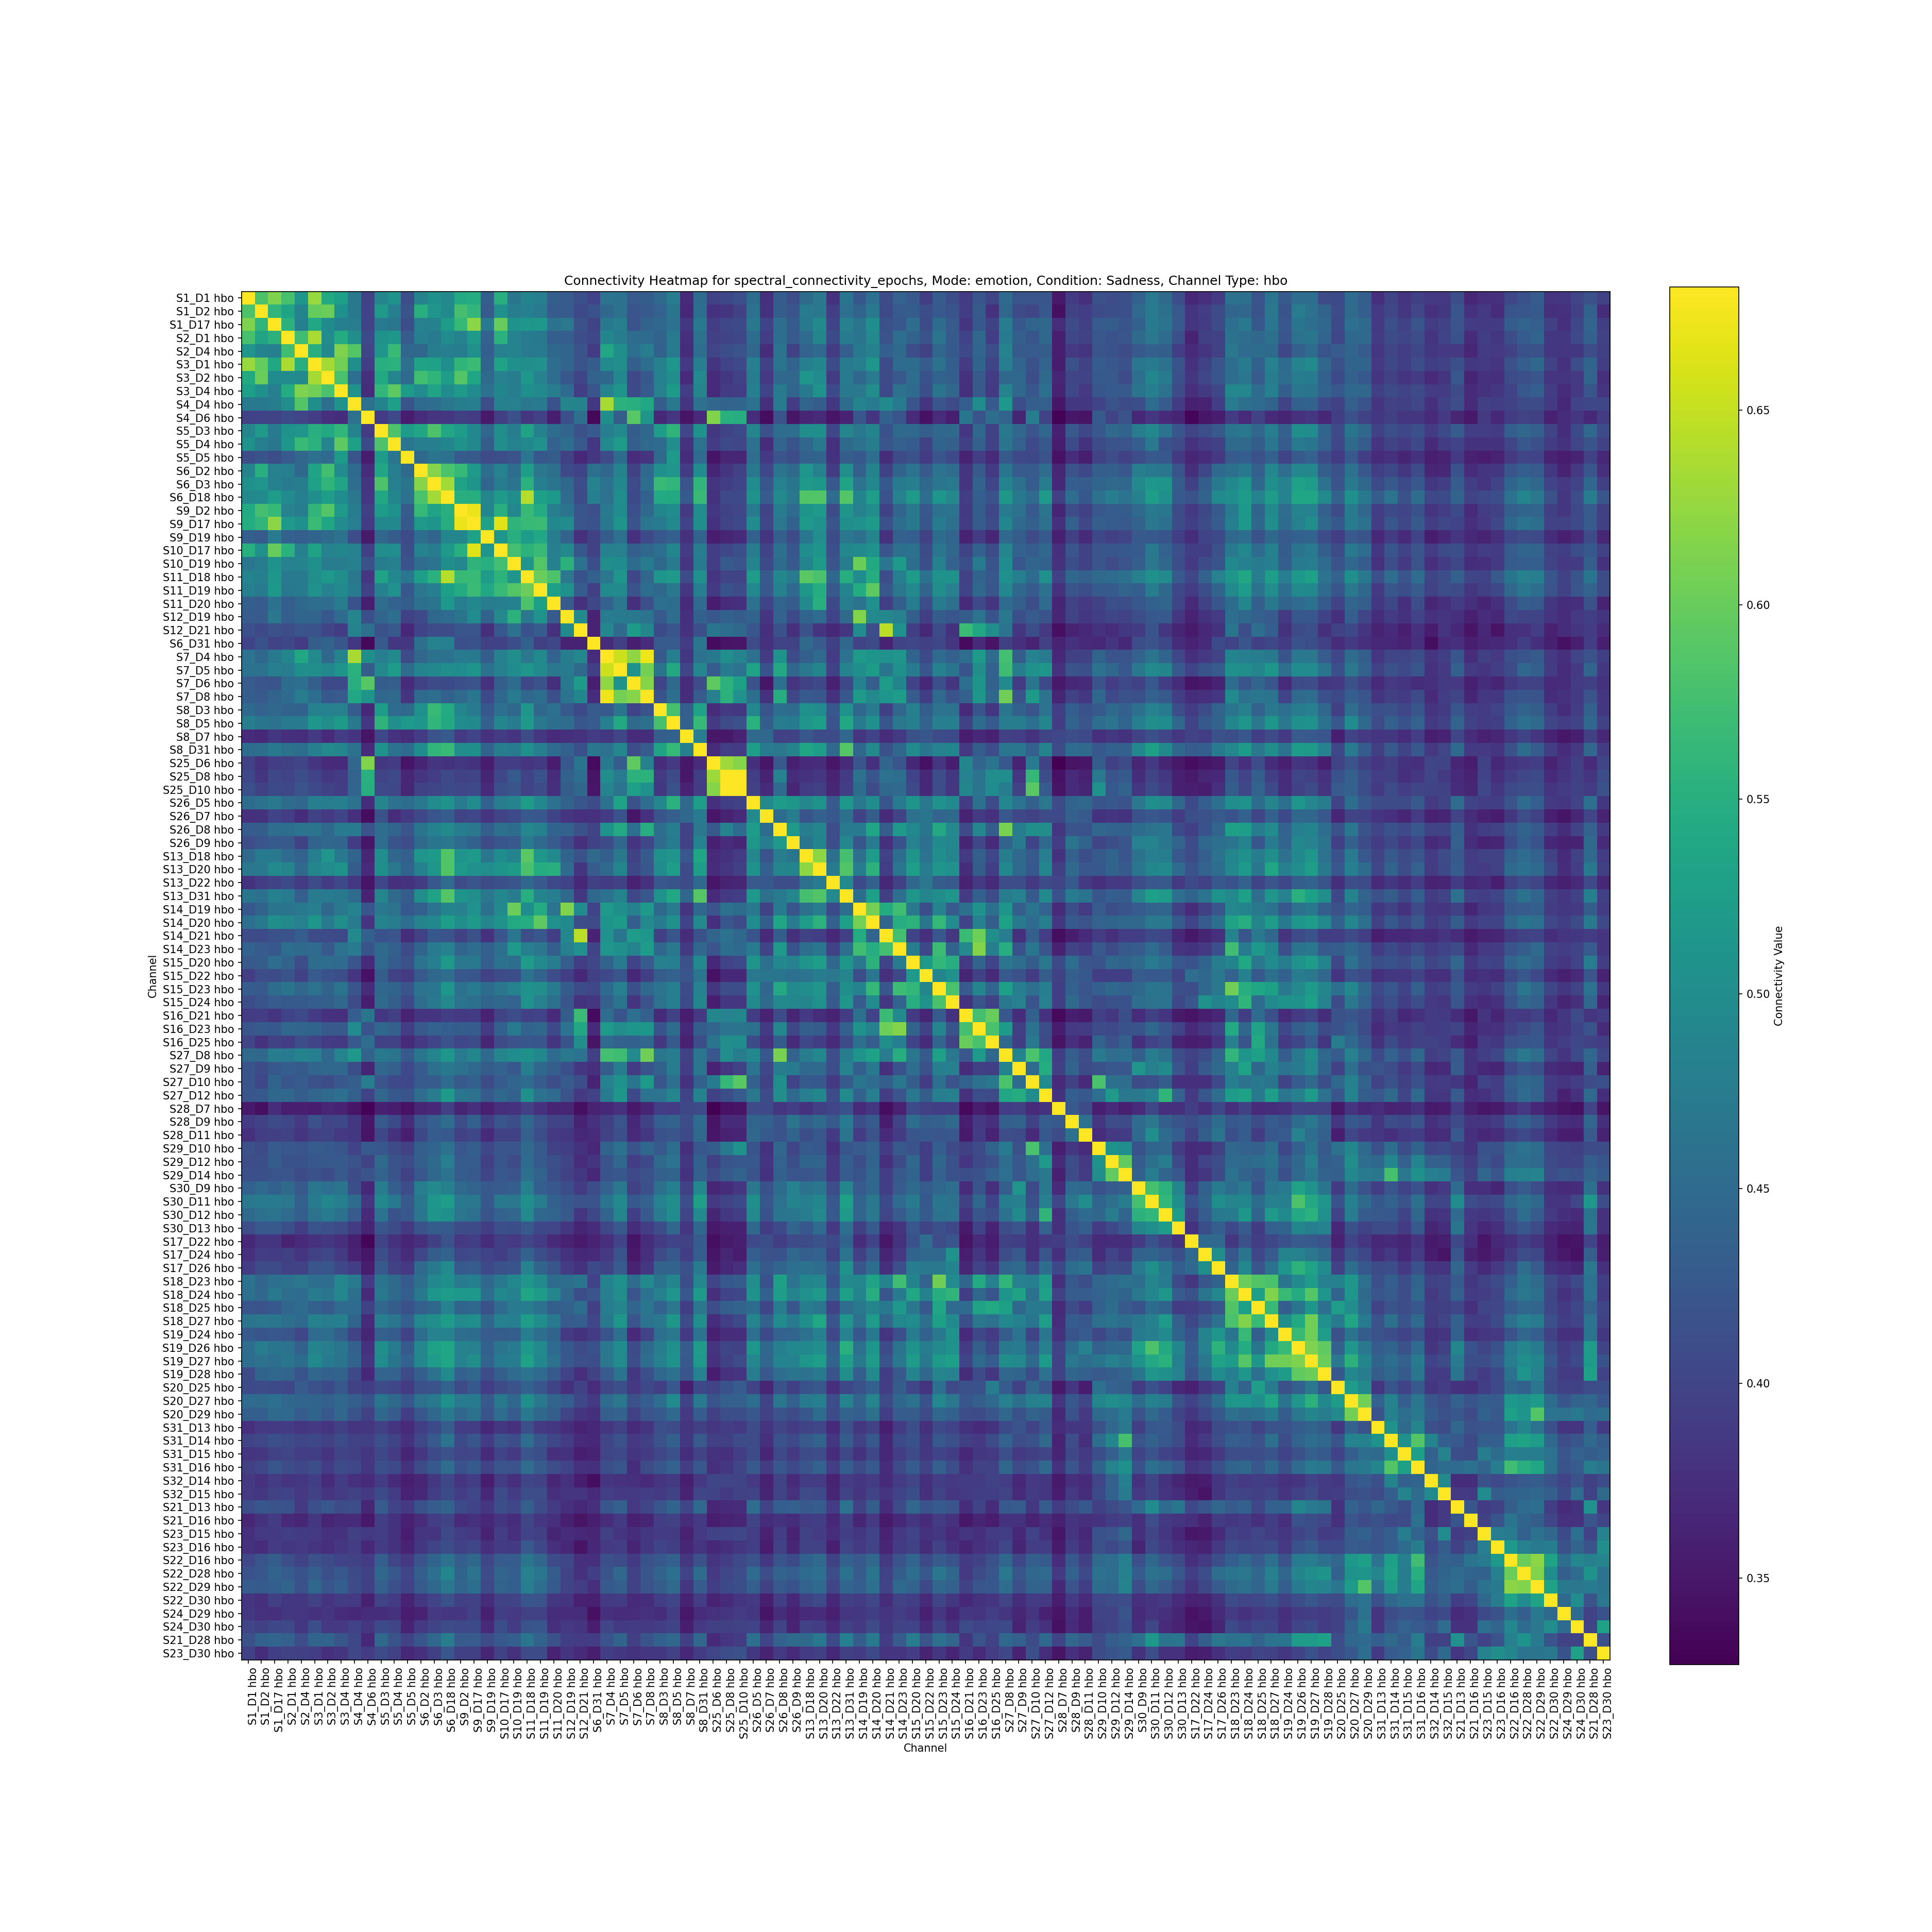
\includegraphics[width=1\textwidth]{C:/Users/super/OneDrive - Ontario Tech University/fNIRS_Emotions/plots/spectral_connectivity_time/chord_plots/conditions/emotion_Sadness_con.png}
    \caption{Example of a chord plot for the condition Sadness, showing the averaged connectivity across participants and epochs between 103 HbT channels (coherence values between 0 and 1).
    The color of the lines represents the coherence value. 
    In general, the brighter the color, the stronger the connectivity between the two channels.}
    \label{fig:chord_plot}
\end{figure}

\subsubsection{Paired Sample t-tests}
For each mode (Face type/Emotion), and pair of conditions (e.g., Joy vs. Fear), individual-level connectivity matrices were extracted, averaging across epochs and time points to obtain, per participant, a symmetric channel-by-channel coherence matrix. 
Because coherence values are bounded between 0 and 1 and exhibit skewed distributions \citep{miranda_de_sa_coherence_2009}, Fisher's r-to-z transform (\texttt{atanh}) was applied to each matrix element to normalize the data prior to parametric testing. 
Paired t-tests for each unique channel pair ($i > j$) were then conducted across participants using SciPy's \texttt{ttest\_rel}.
This directly tests whether mean connectivity differs between conditions, leveraging the paired design to increase statistical sensitivity \citep{hu_characterizing_2023}. 
Given the large number of channel-pair tests, and similar to the GLM analysis above in \ref{sec:contrast_computation}, $p$-values were corrected for FDR using the Benjamini-Hochberg procedure \citep{singh_exploring_2006} with a family-wise error rate of $\alpha$=0.05.

\subsubsection{ROI Chord Plots}
To distill high-dimensional channel-by-channel connectivity into interpretable inter-regional summaries, we mapped individual fNIRS channels onto anatomically defined ROI's. 
This includes left and right frontal, prefrontal, parietal, occipital regions of the brain. 
Since multiple channels may map to the same pair of regions (e.g., several left prefrontal channels connecting to several right occipital channels), we aggregated all significant connections ($p <$ 0.05) between two regions by taking the mean of their t-values. 

\subsection{Memory Task Analysis}
Recall the memory task described in \ref{sec:memory_task}, where participants were asked to indicate whether the 9th face was in the previous block of 8 faces with a 'yes' or 'no' response on the keyboard.
The memory task was not the main focus of the study, but it was used to keep the participants engaged and focused on the faces. 
However, one can investigate whether participants' ability to correctly recognize or recall emotional facial expressions varied depending on the type of face (e.g., real vs. virtual) and the emotion displayed (e.g., happy, sad, angry). 
Raw behavioral data files from the output of the PsychoPy presentation were systematically preprocessed to isolate key response variables. 
For example, if the participant pressed 'y' for yes, and the 9th face was indeed in the previous block, they answered correctly, and if they pressed 'y' for yes, and the 9th face was not in the previous block, they answered incorrectly. 
The same applies for the 'n' for no responses. 
The total correct trials per participant were then summed. 
This data is not subject to the same signal quality criteria as the fNIRS data that was described in \ref{sec:participants}, as it is not a physiological measure. 
Therefore, all 88 participants can be included in the analysis, regardless of their fNIRS signal quality.
However, participants achieving fewer correct responses than 34/56 (e.g., 60\% of trials) were excluded to ensure sufficient engagement in the task, as shown in Figure \ref{fig:correct_responses}.
Only one participant was excluded from the analysis.

\begin{figure}[H]
    \centering
    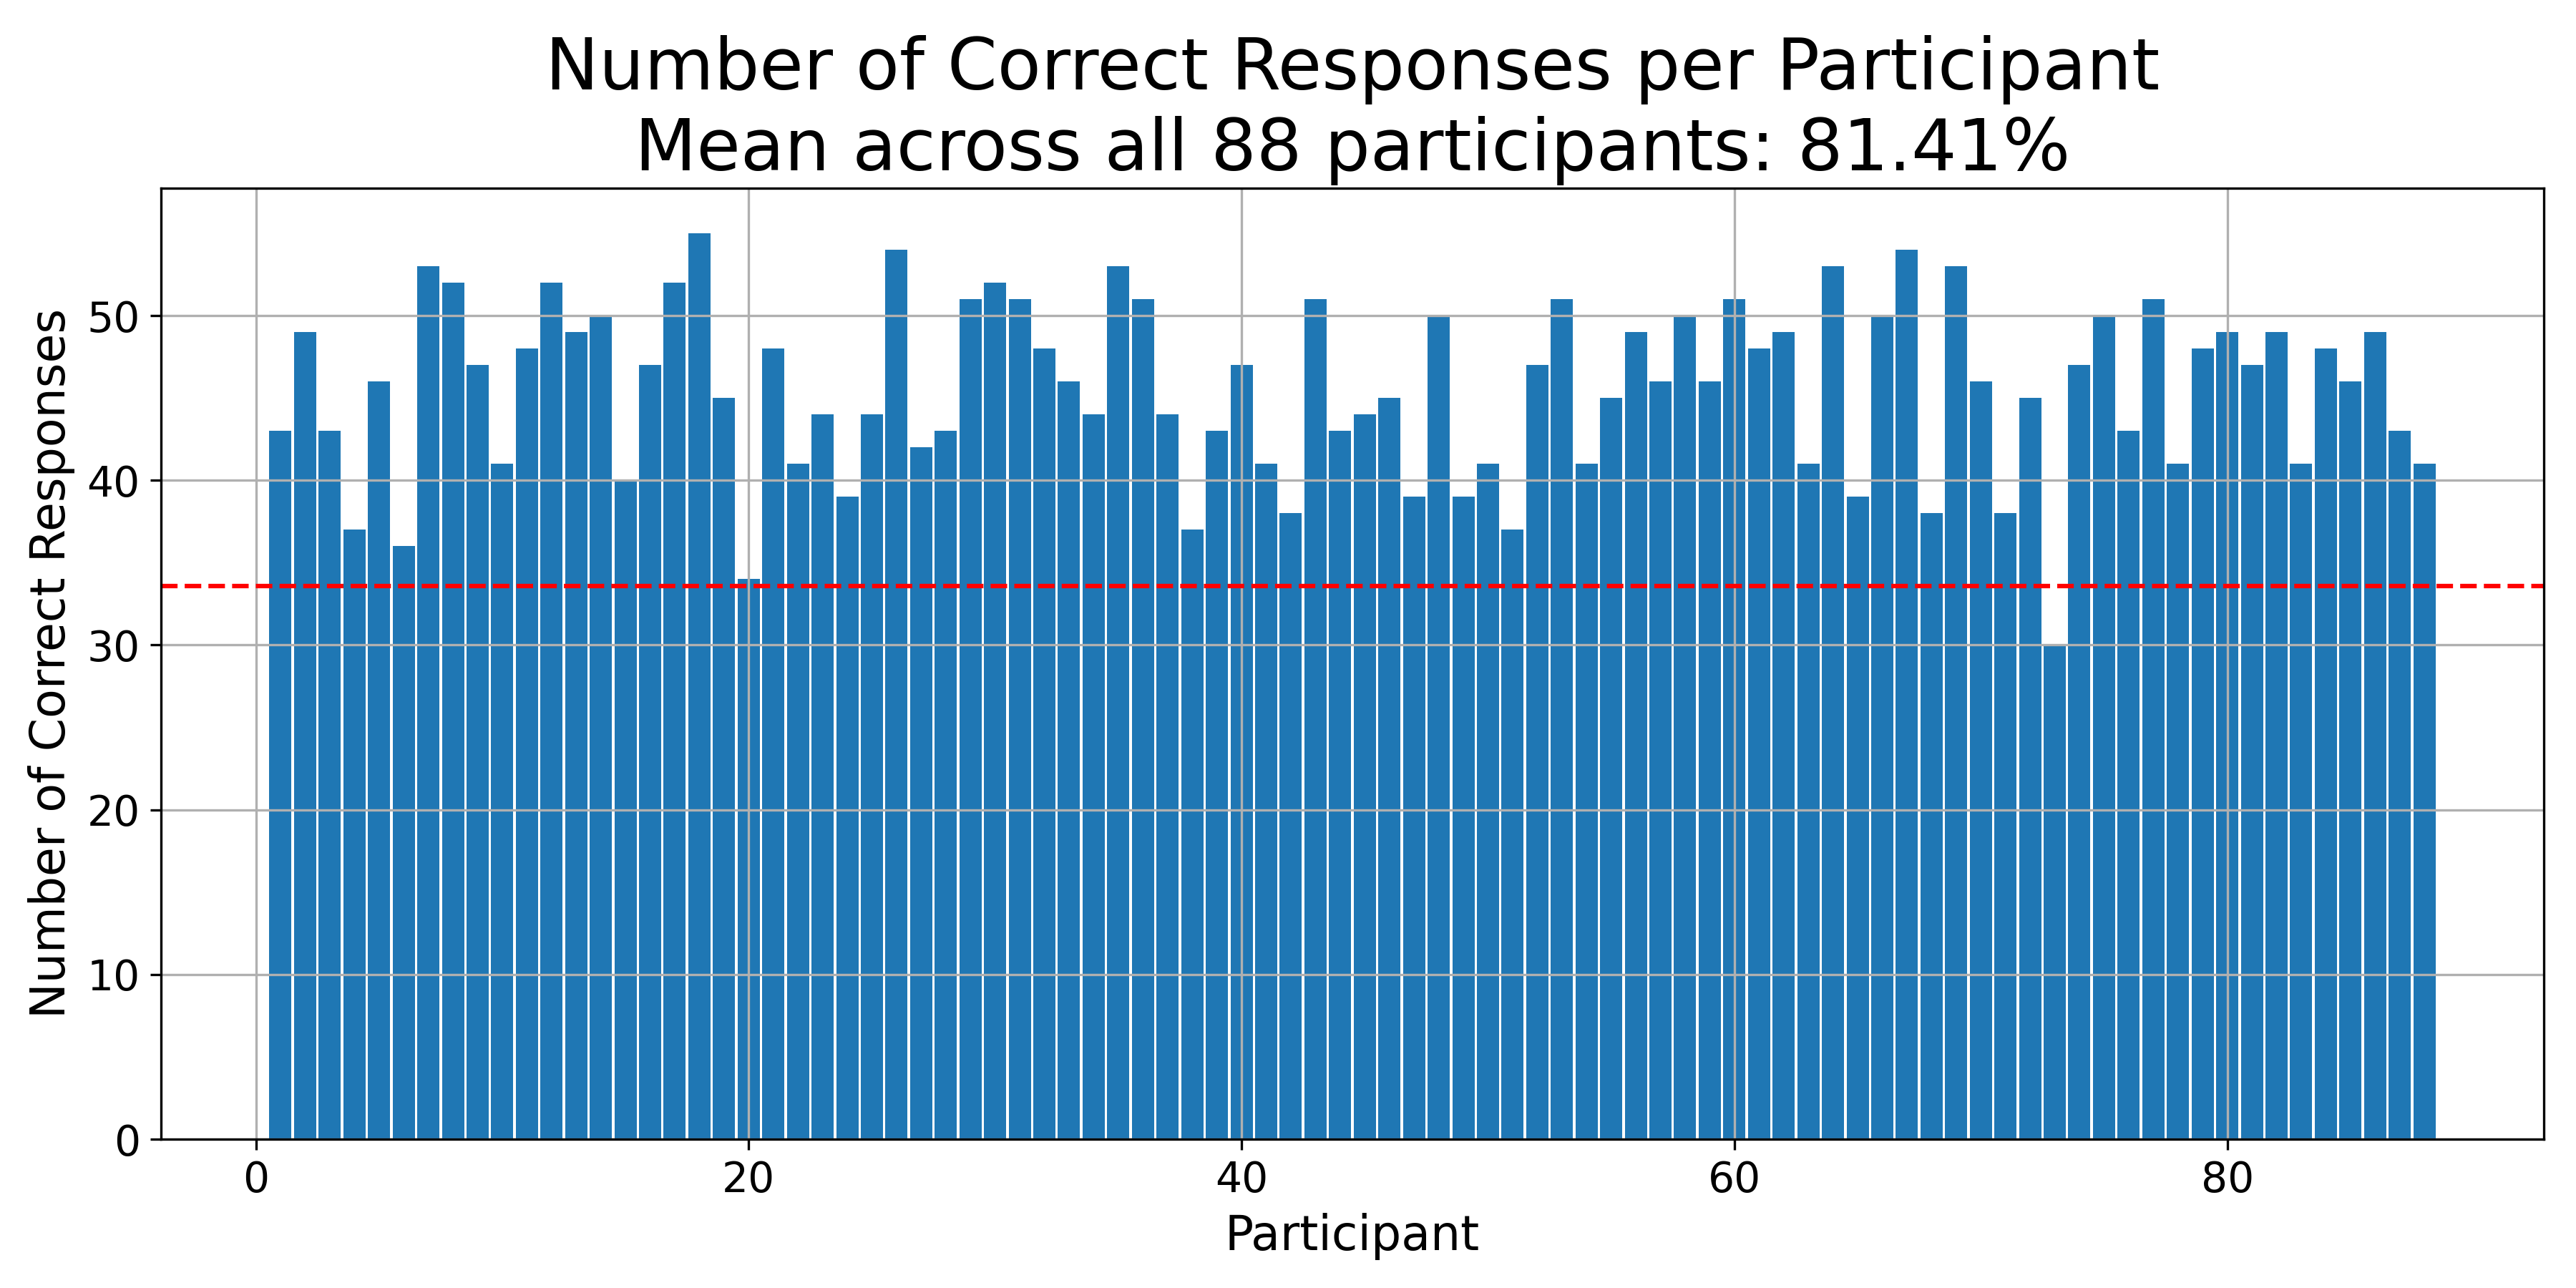
\includegraphics[width=1\textwidth]{C:/Users/super/OneDrive - Ontario Tech University/fNIRS_Emotions/plots/behavioural_responses/correct_responses_by_participant.png}
    \caption{Number of correct responses by participant, the red dashed line represents the threshold of 34/56 correct responses (60\%) that participants must meet to be included in the analysis.
    Only one participant was excluded from the analysis. }
    \label{fig:correct_responses}
\end{figure}

Since each block of faces was either all real or all virtual, and all had the same emotional expression (as discussed in \ref{sec:Procedure}), each y/n response was labeled with Face type and Emotion.
An OLS model was fit with accuracy (converted to numeric 0/1) as the dependent variable and categorical predictors for Face Type, Emotion, and their interaction. 
The goal is to determine the main effects of these two factors individually, as well as their interaction, on response accuracy.
A two-way Type III ANOVA (via \texttt{sm.stats.anova\_lm(model, typ=3)}) provided $F$-statistics and $p$-values for main effects and interaction.
This version of the ANOVA is especially suitable when interactions are included in the model, as it calculates each effect after accounting for all other terms.